\documentclass[11pt]{article}
\usepackage[utf8]{inputenc}
\usepackage[margin=1in]{geometry}
\usepackage{booktabs}
\usepackage{graphicx}
\usepackage{amsmath}
\usepackage{hyperref}
\usepackage{setspace}
\usepackage[english]{babel}
\usepackage{tikz}
\usetikzlibrary{positioning, arrows.meta, shapes.geometric}

\usepackage[
  backend=biber,
  style=apa,
  citestyle=apa,
  natbib=false,
  doi=false,
  isbn=false,
  url=false
]{biblatex}

\addbibresource{../shared/delivery_emission.bib}

% OD flowchart command
\newcommand{\ODFlowchart}{%
  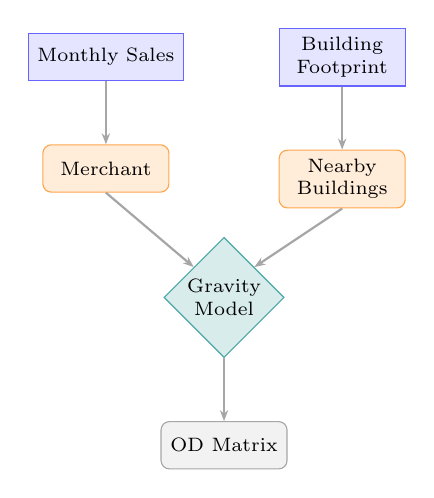
\begin{tikzpicture}[
      node distance=0.6cm and 1.2cm,
      data/.style={rectangle, draw=blue!60, fill=blue!10, minimum width=1.6cm, minimum height=0.6cm, align=center, font=\scriptsize},
      processed/.style={rectangle, draw=orange!70, fill=orange!15, rounded corners=3pt, minimum width=1.6cm, minimum height=0.6cm, align=center, font=\scriptsize},
      output/.style={rectangle, draw=gray!70, fill=gray!10, rounded corners=3pt, minimum width=1.6cm, minimum height=0.6cm, align=center, font=\scriptsize},
      model/.style={diamond, draw=teal!70, fill=teal!15, minimum width=1cm, minimum height=0.8cm, align=center, font=\scriptsize, inner sep=1pt},
      arrow/.style={-{Stealth[scale=0.6]}, thick, draw=gray!70}
    ]
    \node[data] (sales) {Monthly Sales};
    \node[data, right=1.2cm of sales] (building) {Building\\Footprint};
    \node[processed, below=0.8cm of sales] (merchant) {Merchant};
    \node[processed, below=0.8cm of building] (buildings) {Nearby\\Buildings};
    \path (merchant) -- (buildings) coordinate[midway] (mid);
    \node[model, below=0.8cm of mid] (gravity) {Gravity\\Model};
    \node[output, below=0.8cm of gravity] (od) {OD Matrix};
    \draw[arrow] (sales) -- (merchant);
    \draw[arrow] (building) -- (buildings);
    \draw[arrow] (gravity) -- (od);
    \draw[arrow] (merchant.south) -- (gravity.north west);
    \draw[arrow] (buildings.south) -- (gravity.north east);
  \end{tikzpicture}%
}

% Road Distance flowchart command
\newcommand{\RoadDistFlowchart}{%
  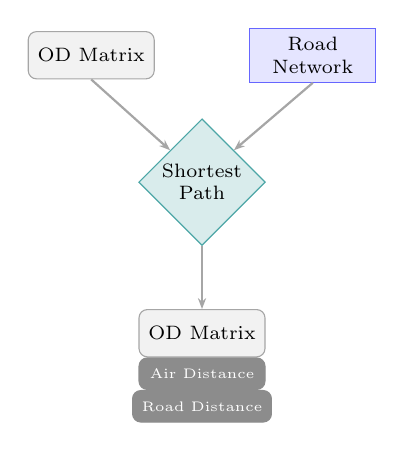
\begin{tikzpicture}[
      node distance=0.6cm and 1.2cm,
      data/.style={rectangle, draw=blue!60, fill=blue!10, minimum width=1.6cm, minimum height=0.6cm, align=center, font=\scriptsize},
      processed/.style={rectangle, draw=orange!70, fill=orange!15, rounded corners=3pt, minimum width=1.6cm, minimum height=0.6cm, align=center, font=\scriptsize},
      output/.style={rectangle, draw=gray!70, fill=gray!10, rounded corners=3pt, minimum width=1.6cm, minimum height=0.6cm, align=center, font=\scriptsize},
      smallbox/.style={rectangle, draw=gray!90, fill=gray!90, text=white, minimum width=1.6cm, minimum height=0.4cm, align=center, font=\tiny, rounded corners=3pt},
      model/.style={diamond, draw=teal!70, fill=teal!15, minimum width=1cm, minimum height=0.8cm, align=center, font=\scriptsize, inner sep=1pt},
      arrow/.style={-{Stealth[scale=0.6]}, thick, draw=gray!70}
    ]
    \node[output] (od) {OD Matrix};
    \node[data, right=1.2cm of od] (roadnet) {Road\\Network};
    \path (od) -- (roadnet) coordinate[midway] (mid);
    \node[model, below=0.8cm of mid] (shortest) {Shortest\\Path};
    \node[output, below=0.8cm of shortest] (result) {OD Matrix};
    \node[smallbox, below=0cm of result.south, anchor=north] (airdist) {Air Distance};
    \node[smallbox, below=0cm of airdist.south, anchor=north] (roaddist) {Road Distance};
    \draw[arrow] (shortest) -- (result);
    \draw[arrow] (od.south) -- (shortest.north west);
    \draw[arrow] (roadnet.south) -- (shortest.north east);
  \end{tikzpicture}%
}

\begin{document}

\begin{titlepage}
  \centering
  \vspace*{1cm}

  {\LARGE\textbf{Research Proposal}}

  \vspace{2cm}

  {\Large\textbf{A Gravity-Based Framework for Scaling Emissions Assessment of Drone and E-Bike Food Delivery Systems}}

  \vspace{2cm}

  {\large Jingxian Lin}\\[0.3cm]
  Department of Civil Engineering\\
  The University of Hong Kong

  \vspace{1.5cm}

  \today

  \vfill

  \begin{tabular}{@{}ll}
    \textbf{Supervisor:} & Dr. Jintao Ke \\[0.5cm]
    \textbf{Signature:} & \includegraphics[height=0.9cm]{signature.png} \\[0.5cm]
  \end{tabular}

  \vspace{1cm}
\end{titlepage}

\newpage
\tableofcontents
\newpage

\section{Introduction}

Unmanned aerial vehicles (UAVs) are emerging as a transformative technology for transportation and logistics, offering fast and flexible delivery with cost-efficient operations. This potential has attracted significant policy attention, with China's Government Work Report highlighting drone delivery in both 2024 and 2025, signaling the strategic importance of the low-altitude economy. Globally, the drone delivery market is forecast to expand from \$3.47 billion in 2025 to \$20.98 billion by 2034, at a compound annual growth rate of 19.45\% \parencite{fortunebi2026drone}.

Food delivery emerges as an ideal application for drone technology. Current drones face constraints in battery capacity and cargo weight, making them best suited for short-distance, last-mile logistics. Food delivery aligns well with these capabilities: orders are typically lighter and smaller than parcels, distances usually remain under 3 km, and the high time sensitivity matches the speed advantage that drones provide.

% Several studies suggest that drones may achieve lower energy consumption and carbon emissions than ground vehicles under certain conditions \parencite{park_comparative_2018, kirschstein_comparison_2020, baldisseri_truck-based_2022}.

The food delivery market in China presents a substantial opportunity for drone adoption. The online food delivery market has grown from approximately 300 billion Yuan in 2017 to over 1 trillion Yuan by 2023 \parencite{statista2024chinafooddelivery}. Leading platforms such as Meituan and Eleme have initiated pilot drone delivery programs in multiple cities, demonstrating early commercial viability.

Despite this growing momentum, the environmental impact of drone delivery systems remains uncertain. The lack of predictive models for evaluating emissions across different urban contexts creates challenges for policymakers and urban planners seeking to determine whether drones truly offer a sustainable advantage over conventional delivery methods, or under which operational conditions drones can offer an environmentally friendly alternative for food delivery.

\section{Literature Review}

A growing body of research has examined the environmental impacts of drone delivery systems, with findings varying substantially depending on comparison vehicles, geographic context, and methodological approach (Table~\ref{tab:lit_review}).

\subsection{Drone vs. Ground Vehicle in Delivery}

Several studies have found drones environmentally favorable compared to traditional diesel delivery vehicles. \textcite{stolaroff_energy_2018} conducted the first empirically calibrated study, finding that small drones achieve significantly lower greenhouse gas emissions than diesel trucks, though warehouse energy requirements can dominate total emissions. Similarly, \textcite{park_comparative_2018} compared drones with motorcycles in South Korea, finding substantially lower drone emissions, with rural areas benefiting significantly more than urban areas from drone adoption. For hybrid configurations, \textcite{baldisseri_truck-based_2022} found that truck-drone systems achieve the lowest emissions across all scenarios tested, but economic viability requires automation to reduce labor costs. Among lighter vehicles, \textcite{rodrigues_drone_2022} demonstrated through empirical flights that only e-cargo bicycles achieve lower emissions per package than drones.

However, these advantages are often conditional on specific operational contexts. \textcite{kirschstein_comparison_2020} employed well-to-wheel energy modeling to demonstrate that drones are competitive only in rural, low-density settings with calm wind conditions. When considering multi-drop routing, \textcite{figliozzi_lifecycle_2017} developed an analytical lifecycle framework showing that while drones are highly energy-efficient per distance, electric tricycles outperform them when multiple customers can be grouped in a single route. Additionally, \textcite{yowtak_comparative_2020} compared drones against battery electric vehicles for grocery delivery, concluding that BEVs outperform drones even for short distances due to payload weight sensitivity.

\subsection{Research Gaps}

Despite this progress, several critical gaps remain. First, most studies compare drones against trucks, vans, or personal vehicles, which are not representative of Asian food delivery where e-bikes dominate. Only \textcite{li_beyond_2025} directly compares drones to e-bikes, finding that the relative advantage depends on the number of orders per trip. Second, existing studies typically rely on aggregate statistical metrics and hypothetical delivery scenarios rather than real origin-destination (OD) order data, which prevents accurate assessment of route-level emission variations across diverse urban environments. Third, few studies have conducted multi-city comparisons across diverse urban contexts to identify the conditions under which drone delivery achieves environmental advantages.

\subsection{Research Objectives}

To address these gaps, this research aims to:
\begin{enumerate}
  \item Develop a gravity-based food delivery demand generation method that produces door-to-door order data, enabling more precise analysis than conventional zone-based or aggregate approaches.
  \item Present the first comprehensive comparison of carbon emissions between e-bike and drone delivery systems across multiple cities in China.
  \item Identify key urban features (e.g., population density, terrain, delivery distance distribution) that determine when drone delivery achieves lower emissions, providing actionable insights for sustainable logistics planning.
\end{enumerate}

\begin{table}[h]
  \centering
  \caption{Comparison of drone delivery emission studies}
  \label{tab:lit_review}
  \begin{tabular}{l l c c c c}
    \toprule
    \textbf{Study} & \textbf{Comparison} & \textbf{Greener?} & \textbf{OD Data} & \textbf{Scale} & \textbf{Method} \\
    \midrule
    \textcite{figliozzi_lifecycle_2017} & Van/Tricycle & Mixed & No & Analytical & LCA \\
    \textcite{park_comparative_2018} & Motorcycle & Yes & No & Two regions (Korea) & LCA \\
    \textcite{stolaroff_energy_2018} & Truck & Mixed & No & National (USA) & LCA \\
    \textcite{kirschstein_comparison_2020} & Truck & Mixed & No & Single city (Germany) & Use-phase \\
    \textcite{yowtak_comparative_2020} & ICEV/BEV & Mixed & No & Single city (USA) & LCA \\
    \textcite{baldisseri_truck-based_2022} & Truck & Yes & No & Suburban (Italy) & LCA \\
    \textcite{rodrigues_drone_2022} & Car/Van/Bike & Mixed & No & National (USA) & Use-phase \\
    \textcite{li_beyond_2025} & E-bike & Mixed & No & Single city (China) & LCA \\
    \midrule
    \textbf{This work} & \textbf{E-bike} & \textbf{Yes} & \textbf{Yes} & \textbf{National (China)} & \textbf{LCA} \\
    \bottomrule
  \end{tabular}
\end{table}

\section{Methodology}

\subsection{Data Sources}

\textbf{Monthly Sales Data:} The dataset includes latitude, longitude, and monthly sales data for 1,075,362 valid takeout merchants across China, collected in August 2021 from the Meituan Takeaway platform.

\textbf{Building Footprint Data:} Building polygons, heights, and LoD1 3D models are obtained from the Global Building Atlas, which provides global coverage containing 2.75 billion buildings at 3m resolution \parencite{zhu_globalbuildingatlas_2025}.

\textbf{Road Network Data:} Street network data is retrieved from OpenStreetMap \parencite{openstreetmap} via the OSMnx library, including all road types except motorways. This network is used to compute e-bike delivery distances along routes accessible to non-motorized vehicles.

\subsection{OD Generation}

The proposed framework generates origin-destination pairs by first processing sales data to extract merchants, then identifying nearby buildings from footprint data, and finally applying a gravity model to distribute demand (Figure~\ref{fig:od_flowchart}).

\begin{figure}[h]
  \centering
  \ODFlowchart
  \caption{OD generation flowchart}
  \label{fig:od_flowchart}
\end{figure}

Under the assumption that larger buildings attract more orders due to higher population density while greater distances reduce demand owing to increased delivery time and cost, the gravity model is formulated as follows. The estimated number of deliveries $D_{ij}$ from origin $i$ to destination $j$ is the total demand $P_i$ at origin $i$ multiplied by the proportion of attraction that destination $j$ exerts relative to all destinations:
\begin{equation}
  D_{ij} = P_{i} \cdot \frac{f(d_{ij}, v_{j})}{\sum_{j \in \mathcal{D}} f(d_{ij}, v_{j})}, \quad \forall i \in \mathcal{O}, j \in \mathcal{D}
\end{equation}

The attraction function $f$ is defined such that $v_j^\alpha$ represents the attraction of destination $j$ based on building volume, while $d_{ij}^\beta$ captures the distance decay effect:
\begin{equation}
  f(d_{ij}, v_{j}) = \frac{v_{j}^\alpha}{d_{ij}^{\beta}}
\end{equation}

Here, $\mathcal{O}$ is the set of origins, $\mathcal{D}$ is the set of destinations, and $\alpha$ and $\beta$ are elasticity coefficients.

The model parameters are calibrated as $\alpha = 1.7$ and $\beta = 0.5$, validated against descriptive statistical indicators showing that the mean delivery distance per express food order in first-tier cities is 2.23 km \parencite{xie_environmental_2021}.

\subsection{Road Distance Calculation}

For each OD pair, both straight-line (Euclidean) distance and road network distance are computed (Figure~\ref{fig:road_dist_flowchart}). Since the road network is represented as a graph where nodes correspond to intersections and edges correspond to road segments, the coordinates of merchants and customers must first be mapped to their nearest network nodes. This spatial mapping is accelerated using a KD-tree data structure, which reduces query time complexity from $O(n)$ to $O(\log n)$.

Once both endpoints are assigned to network nodes, the shortest path distance is computed using Dijkstra's algorithm. To further improve computational efficiency, unique origin-destination node pairs are identified first, ensuring that the shortest path calculation is performed only once for each distinct pair of intersections. This deduplication typically reduces computation time by approximately 50\%.

\begin{figure}[h]
  \centering
  \RoadDistFlowchart
  \caption{Road distance calculation flowchart}
  \label{fig:road_dist_flowchart}
\end{figure}

\subsection{Emission Models}

The total lifecycle carbon emissions for each delivery mode consist of two components: production and disposal emissions, and use-phase emissions:
\begin{equation}
  CO_2e_{total} = CO_2e_{pro+dis} + CO_2e_{use}
\end{equation}

\subsubsection{Lifecycle Emission Model}

Production and disposal emissions include body manufacturing, battery production, and end-of-life disposal. Both e-bikes and drones follow the same structural formula. For e-bikes:
\begin{equation}
  CO_2e_{E_{pro+dis}} = e_{E_m} \times w_{E_m} + e_{E_b} \times V_{E_b} \times n_{E_b} + e_{E_{md}} \times w_{E_m} + e_{E_{bd}} \times V_{E_b} \times n_{E_b}
\end{equation}
and for drones:
\begin{equation}
  CO_2e_{U_{pro+dis}} = e_{U_m} \times w_{U_m} + e_{U_b} \times V_{U_b} \times n_{U_b} + e_{U_{md}} \times w_{U_m} + e_{U_{bd}} \times V_{U_b} \times n_{U_b}
\end{equation}
where $e_m$ and $e_{md}$ are the production and disposal emission factors for the vehicle body with mass $w_m$, and $e_b$ and $e_{bd}$ are the production and disposal emission factors for batteries with capacity $V_b$ and replacement count $n_b$. While the formula structure is identical, the parameter values differ significantly: drones have lower body weight but higher battery emission factors due to lithium polymer chemistry, and their shorter battery lifespans require more frequent replacements.

These production emissions are allocated to each delivery by dividing the total by the estimated lifetime number of deliveries. The lifetime deliveries are estimated from daily working hours, delivery time per trip (which depends on distance and velocity), working days per year, and vehicle lifespan. Drones typically achieve higher lifetime deliveries due to faster speeds and longer daily operating hours, which spreads their production emissions across more orders. Battery replacement cycles are also considered, with battery-related emissions amortized over the shorter battery lifespan rather than the vehicle lifespan.

\subsubsection{Use-phase Emission Model}

Use-phase emissions are calculated from the power consumption during delivery. For e-bikes:
\begin{equation}
  CO_2e_{E_{use}} = e_{E_c} \times P_{E} \times \sum_{i=1}^{m_E} (d_{E_i} / v_E)_i
\end{equation}
where $e_{E_c}$ is the grid emission factor, $P_E$ is the e-bike power, and $\sum (d_{E_i} / v_E)_i$ is the total travel time to complete $m_E$ orders. The e-bike power model calculates the instantaneous mechanical power as:
\begin{equation}
  P_{E} = P_{\text{rolling}} + P_{\text{air}} + P_{\text{grade}} + P_{\text{acc}}
\end{equation}
where rolling resistance captures the friction between tires and road surface (proportional to vehicle mass), aerodynamic drag represents air resistance (increasing with the cube of velocity), grade climbing accounts for the power needed to overcome gravity on inclines, and acceleration reflects the power required for speed changes during stop-and-go urban delivery.

For drones, use-phase emissions account for both level flight and vertical climb:
\begin{equation}
  CO_2e_{U_{use}} = e_{U_c} \times \left[ P_{U_L} \times \sum_{i=1}^{m_U} (d_{L_i} / v_{U_L})_i + P_{U_T} \times \sum_{i=1}^{m_U} (h_{T_i} / v_{U_T})_i \right]
\end{equation}
where $P_{U_L}$ is the level flight power, $P_{U_T}$ is the climb power, $\sum (d_{L_i} / v_{U_L})_i$ is the total level flight time, and $\sum (h_{T_i} / v_{U_T})_i$ is the total climb time. The drone power model calculates the power required for multi-rotor flight as:
\begin{equation}
  P_{U} = P_{\text{induced}} + P_{\text{profile}} + P_{\text{drag}} + P_{\text{climb}} + P_{\text{aux}}
\end{equation}
where induced power is required to generate rotor thrust for lift, profile power is lost to blade drag as rotors spin, parasitic drag arises from air resistance on the aircraft body during forward flight, climb power provides the additional thrust for vertical ascent, and auxiliary power supplies onboard electronics including the flight controller, GPS, and communication systems.

\subsection{Emission Reduction Analysis}

To identify optimal deployment strategies for hybrid drone-e-bike delivery systems, a threshold-based assignment approach is employed. The relative emission performance of drones versus e-bikes depends on two key factors: delivery distance and detour ratio (the ratio of road distance to straight-line distance). These factors exhibit an inverse trade-off relationship: at shorter distances, drones require a higher detour ratio to outperform e-bikes, while at longer distances, even modest detour ratios favor drone delivery. Consequently, drones become environmentally favorable when either delivery distance is high, detour ratio is high, or both.

The analysis proceeds by defining a distance threshold $d^*$ that determines mode assignment: deliveries with road distance greater than or equal to $d^*$ are assigned to drones, while those below the threshold are handled by e-bikes. A range of candidate thresholds is generated based on the observed road distance distribution, spanning from the 5th to the 95th percentile. For each threshold value, the total lifecycle emissions of the resulting mixed fleet are computed by summing the per-order emissions across all deliveries. The optimal threshold is identified as the value that minimizes total emissions, or equivalently, maximizes emission reduction relative to an all-e-bike baseline. From this optimal threshold, the corresponding drone ratio—the proportion of deliveries assigned to drones—is derived, providing actionable guidance for fleet composition decisions.

\section{Preliminary Results and Expected Outcomes}

To illustrate the proposed methodology, we present preliminary results from Luohu District, Shenzhen. The gravity model generates 552,635 valid OD pairs with an average road distance of 2.29~km and an average detour ratio of 1.53. Under the all-e-bike scenario, total annual lifecycle emissions are estimated at 41.4 tonnes CO$_2$e, while the all-drone scenario reduces this to 30.8 tonnes CO$_2$e---a 25.5\% reduction. Applying threshold-based assignment with an optimal distance threshold of 0.72~km (assigning 87.8\% of deliveries to drones) achieves a maximum reduction of 29.8\%, representing an additional 4.3 percentage points improvement over all-drone deployment.

Analysis across seven Chinese districts demonstrates that emission reduction potential varies substantially with local conditions, ranging from 23\% (Gulou, Nanjing) to 65\% (Pudong, Shanghai). Sensitivity analysis reveals that drone delivery becomes increasingly favorable as delivery distance increases and detour ratio rises, with the breakeven point shifting toward shorter distances when road networks are more circuitous. Initial correlation analysis suggests that optimal drone deployment ratio is positively associated with total road network length (r=0.79), while maximum emission reduction correlates with average detour ratio (r=0.66) and average road distance (r=0.73). Further analysis will extend these findings to additional cities to develop robust predictive models for sustainable logistics planning.

% \section{Contributions}

% This research makes the following contributions:

% \begin{enumerate}
%   \item \textbf{Methodological:} A gravity-based OD generation framework that produces door-to-door delivery demand data, enabling spatially explicit emission analysis at unprecedented scale.

%   \item \textbf{Empirical:} The first comprehensive, country-scale comparison of carbon emissions between e-bike and drone food delivery systems across multiple Chinese cities with diverse urban characteristics.

%   \item \textbf{Practical:} Identification of key urban features that determine when drone delivery achieves lower emissions, providing actionable insights for sustainable urban logistics planning and policy-making.
% \end{enumerate}

% \section{Research Timeline}

% \begin{table}[h]
%   \centering
%   \caption{Proposed research timeline}
%   \begin{tabular}{l l}
%     \toprule
%     \textbf{Phase} & \textbf{Activities} \\
%     \midrule
%     Phase 1 & Data collection and preprocessing \\
%     Phase 2 & OD generation framework development \\
%     Phase 3 & Emission model implementation and validation \\
%     Phase 4 & Multi-city analysis and comparison \\
%     Phase 5 & Urban feature correlation analysis \\
%     Phase 6 & Thesis writing and publication \\
%     \bottomrule
%   \end{tabular}
% \end{table}

\section{Conclusion}

This research proposes a comprehensive framework for assessing the environmental implications of drone versus e-bike food delivery systems. By developing a gravity-based OD generation method and applying lifecycle emission models across multiple Chinese cities, this study will provide evidence-based insights into the conditions under which drone delivery offers environmental advantages. The findings will contribute to sustainable urban logistics planning and inform policy decisions regarding emerging delivery technologies.

\printbibliography

\end{document}
